\documentclass[11pt]{article}

\usepackage[margin=1.05in]{geometry}
\usepackage[T1]{fontenc}
\usepackage{lmodern}
\usepackage{microtype}
\usepackage{amsmath,amssymb,amsthm,mathtools}
\usepackage{booktabs,tabularx,array}
\usepackage{enumitem}
\usepackage[dvipsnames]{xcolor}
\usepackage{tikz}
\usetikzlibrary{arrows.meta,calc,positioning,shapes.geometric}
\usepackage{fancyhdr}
\usepackage[colorlinks=true,linkcolor=MidnightBlue,citecolor=MidnightBlue,urlcolor=MidnightBlue]{hyperref}

\definecolor{ink}{HTML}{18212B}
\definecolor{muted}{HTML}{586574}
\definecolor{redpt}{HTML}{C94A49}
\definecolor{bluept}{HTML}{3979B8}
\definecolor{warm}{HTML}{FFF4DF}
\definecolor{cool}{HTML}{EEF5FB}
\definecolor{linegray}{HTML}{B6C0CA}

\color{ink}
\setlength{\parskip}{0.35em}
\setlist{nosep,leftmargin=1.6em}
\renewcommand{\arraystretch}{1.15}
\newcolumntype{Y}{>{\raggedright\arraybackslash}X}

\pagestyle{fancy}
\fancyhf{}
\fancyhead[L]{\small\color{muted}The optimal two-colour six-point constant}
\fancyhead[R]{\small\color{muted}\thepage}
\renewcommand{\headrulewidth}{0.35pt}

\theoremstyle{plain}
\newtheorem{theorem}{Theorem}[section]
\newtheorem{lemma}[theorem]{Lemma}
\newtheorem{proposition}[theorem]{Proposition}
\newtheorem{corollary}[theorem]{Corollary}
\theoremstyle{definition}
\newtheorem{definition}[theorem]{Definition}
\newtheorem{conjecture}{Conjecture}
\theoremstyle{remark}
\newtheorem{remark}[theorem]{Remark}

\newcommand{\R}{\mathbb R}
\newcommand{\Z}{\mathbb Z}
\newcommand{\HH}{\mathcal H}
\newcommand{\score}{\operatorname{score}}
\newcommand{\diam}{\operatorname{diam}}
\newcommand{\dist}{\operatorname{dist}}
\newcommand{\sstar}{s_{\!*}}
\newcommand{\cstar}{c_{\!*}}
\newcommand{\W}{\mathcal W}
\newcommand{\lowdens}{\Theta^{1}_{*}}

\title{\bfseries The optimal two-colour six-point constant\\[0.3em]
\large for Besicovitch's $1/2$ problem}
\author{Yongxi Lin}
\date{September 2026}

\begin{document}
\maketitle

\begin{abstract}
Besicovitch's $1/2$ conjecture asserts that a planar Borel set of finite
$\HH^1$ measure whose lower density exceeds $1/2$ almost everywhere is
countably $1$-rectifiable.  Following the linear-programming strategy
introduced by De Lellis, Glaudo, Massaccesi and Vittone, the conjecture is
attacked through a family of finite packing problems whose optimal
constants bound the true density threshold from above.  We solve the
two-colour, six-centre instance of that family exactly.  Its optimal
constant is the algebraic number
\[
 \theta_6=\sstar=0.693306421825904872690678414403710951\ldots,
\]
specified by an isolated pair of radical equations rather than by a
decimal, and the extremal configuration is unique up to the evident
symmetries.  Combined with a direct six-centre transfer to the Besicovitch
pair condition and the standard rectifiability machinery, this gives the
bound $\sigma_1(\R^2)\le\sstar$ for the planar rectifiability threshold.
The proof is computer-assisted only in explicitly isolated geometric
inequalities: every certificate is a finite, outward-rounded interval
computation over rational data, and no floating-point sign, hash, or exit
code is a proof object.  A companion Lean~4 development formalizes the
argument; its present status is described in Section~\ref{sec:lean}.
\end{abstract}

\tableofcontents

\section{Introduction}\label{sec:intro}

\subsection{The problem}

Let $E\subset\R^2$ be a Borel set with $\HH^1(E)<\infty$, where $\HH^1$
denotes $1$-dimensional Hausdorff measure.  The \emph{lower density} of $E$
at a point $x$ is
\[
 \lowdens(E,x)=\liminf_{r\downarrow0}\frac{\HH^1(E\cap B(x,r))}{2r},
\]
the normalization $2r$ being the diameter of the ball, so that a straight
segment has density $1$ at its interior points.  The set $E$ is
\emph{countably $1$-rectifiable} if $\HH^1$-almost all of it can be covered
by countably many Lipschitz curves.

A classical theorem of Besicovitch says that a set with lower density
strictly larger than $3/4$ almost everywhere is rectifiable, and he
conjectured that $3/4$ can be replaced by $1/2$.

\begin{conjecture}[Besicovitch's $1/2$ conjecture]
If $E\subset\R^2$ is Borel with $\HH^1(E)<\infty$ and
$\lowdens(E,x)>1/2$ for $\HH^1$-a.e.\ $x\in E$, then $E$ is countably
$1$-rectifiable.
\end{conjecture}

The threshold $1/2$ is the natural one: it is the value attained at the
endpoint of a segment, and no known construction of a purely
$1$-unrectifiable set of finite length achieves a lower density above it.

It is convenient to name the optimal constant.  Write
\[
 \sigma_1(\R^2)
 =\inf\bigl\{\beta\ge0:\
 \text{every finite-measure Borel set with }\lowdens\ge\beta\ \text{a.e.\ is
 countably $1$-rectifiable}\bigr\}.
\]
Besicovitch's conjecture is the assertion $\sigma_1(\R^2)=1/2$.

\subsection{History}

The recorded progress on the upper bound for $\sigma_1(\R^2)$ is short and
hard-won.

\begin{center}
\begin{tabularx}{\textwidth}{@{}llY@{}}
\toprule
year & bound & source\\
\midrule
1928 & $1-10^{-2576}$ & Besicovitch\\
1938 & $3/4$ & Besicovitch\\
1992 & $(2+\sqrt{46})/12=0.73186\ldots$ & Preiss and Ti\v{s}er\\
2024 & $0.7$ & De Lellis, Glaudo, Massaccesi and Vittone\\
\bottomrule
\end{tabularx}
\end{center}

The 1992 bound of Preiss and Ti\v{s}er stood for more than three decades.
Its method rests on a two-point inequality for straight measures, and the
sharp threshold obtainable from that method is the unique positive root of
$8s^3+4s^2-3s-3$, namely $0.72655\ldots$.

The decisive structural advance is due to De~Lellis, Glaudo, Massaccesi and
Vittone, who recast the problem as a family of finite-dimensional
optimization problems.  Their insight is that the passage from a density
hypothesis to rectifiability can be routed through a purely finite
statement about disjoint balls centred at finitely many points, and that
this finite statement is a linear program once the centres are fixed.  The
optimization approach in the present work, and in the accompanying Lean
development, is directly inspired by theirs.

\subsection{What is proved here}

The finite problems in this family are indexed by the number of centres and
by how those centres are grouped.  The instance solved here uses two
\emph{colours} --- corresponding to the two sets $E_1,E_2$ that a
separation argument produces --- and three centres of each colour: a root
and two children.  Six centres in all.  Write $\theta_6$ for the optimal
constant of that instance; a precise definition is given in
Section~\ref{sec:problem}.

\begin{theorem}[Main theorem; Theorem~\ref{thm:main-body}]\label{thm:A}
The optimal two-colour six-point constant is the algebraic number
\[
 \theta_6=\sstar=0.693306421825904872690678414403710951\ldots,
\]
described exactly in Section~\ref{sec:number}.  The normalized extremal
configuration is unique up to reflection in the root line, interchange of
the colours, and relabelling of the two children within either colour.
\end{theorem}

The constant is not a numerical artefact of an optimizer.  It is pinned by
two radical equations inside an explicit rational isolation box, and the
decimal expansion above appears nowhere in the proof.  What makes it that
particular number is that three distinct packing mechanisms tie there
simultaneously; this is explained in Section~\ref{sec:intuition}.

\begin{theorem}[Transfer; Section~\ref{sec:transfer}]\label{thm:B}
$\sigma_1(\R^2)\le\sstar$.
\end{theorem}

Theorem~\ref{thm:B} follows from Theorem~\ref{thm:A} by a direct six-centre
argument establishing the Besicovitch pair condition at every parameter
$\beta>\sstar$, followed by the passage from that condition to
rectifiability and an infimum.  Both steps are described in
Section~\ref{sec:transfer} and are fully formalized.

\subsection{Where a computer is used}

Three ingredients of the proof are finite interval computations:

\begin{enumerate}
\item the isolation of the algebraic endpoint and its associated weights;
\item a list of strict routing separators that prune the case tree;
\item the two analytic inequalities of Section~\ref{sec:weighted}, namely a
      self inequality on one sibling pair and a contraction inequality
      relating a mixed pair to the two self terms.
\end{enumerate}

In every case the statement being certified is a \emph{universal
inequality on an explicitly covered compact domain}, not the output of an
optimizer.  All interval endpoints are rational or dyadic, every arithmetic
operation is rounded outward using integers, and every sign decision is an
integer comparison.  No random sampling, floating-point comparison,
\texttt{native\_decide}, or unchecked external computation enters a proof
step.  Section~\ref{sec:certificates} describes the arithmetic, the charts,
and the exact domains covered.

\subsection{Organization}

Sections~\ref{sec:outline} and~\ref{sec:intuition} are, respectively, a
roadmap of the argument and an informal account of the geometry behind it;
a reader who wants to know what the proof does, and why the answer is what
it is, should be able to stop after them.  The details begin in
Section~\ref{sec:problem}.  Section~\ref{sec:number} constructs the exact
endpoint, Section~\ref{sec:obstruction} proves the lower obstruction,
Sections~\ref{sec:nine} and~\ref{sec:weighted} prove the converse,
Section~\ref{sec:optimality} assembles Theorem~\ref{thm:A},
Section~\ref{sec:certificates} documents the certificates,
Section~\ref{sec:transfer} deduces Theorem~\ref{thm:B}, and
Section~\ref{sec:lean} reports on the formalization.  Three appendices
collect the routing algebra, the rational tangent lemma, and the exact
weights.

\section{Outline of the proof}\label{sec:outline}

The whole argument is a chain of five reductions.  None of them is long to
state; the work is in the last two.

\paragraph{Step 1: from density to a straight measure and a separated
pair.}
Suppose $E$ is a counterexample.  Standard measure-theoretic surgery ---
decomposition into rectifiable and purely unrectifiable parts,
differentiation, and rescaling --- replaces $E$ by a \emph{straight}
measure $\mu$, one for which every measurable set $A$ satisfies
$\mu(A)\le\diam A$, still with lower density above the threshold almost
everywhere.  Inside such a measure one selects two measurable sets
$E_1,E_2$ at small positive distance, and asks whether some open set
meeting both must carry a definite amount of mass \emph{outside}
$E_1\cup E_2$.  That question is the Besicovitch pair condition; if it has
a positive answer at a parameter $\beta$, then $\beta$ forces
rectifiability.

\paragraph{Step 2: from the pair condition to a finite packing problem.}
Pick approximate closest points of $E_1$ and $E_2$ and normalize their
distance to $1$.  Straightness converts the mass in the unit ball around
each of these two points into a \emph{sibling pair}: two further points of
the same set, at mutual distance at least $2s$, each within distance $1$ of
its own root.  This is exactly six points, in two colours of three.  If for
every such six-point configuration one can exhibit a family of balls whose
total radius is at least $1/(2s)$ times the diameter of their union, then
inclusion--exclusion against straightness produces the required leaking open
set, and the pair condition holds for every $\beta>s$.

\paragraph{Step 3: the finite problem, and its optimal constant.}
The finite problem is therefore: for which $s$ does every admissible
six-point configuration admit a \emph{packing move} --- a choice of at least
one centre of each colour and radii, with same-colour balls disjoint --- of
nonnegative \emph{score}
\[
 \score_s=\sum_i r_i-\frac{D}{2s},\qquad D=\diam\Bigl(\bigcup_i \bar B(x_i,r_i)\Bigr)?
\]
The optimal constant $\theta_6$ is the infimum of such $s$.  Since the
transfer of Step~2 needs only $\beta>s$, the value $\theta_6$ itself is
what bounds $\sigma_1(\R^2)$.

\paragraph{Step 4: the lower obstruction.}
One exhibits a single configuration $X_*$ for which no move has positive
score at $s=\sstar$ and every move has negative score below it.  There are
$49$ possible supports; for each, the choice of radii is a linear program,
so a feasible dual for each support certifies the claim exactly.  Five
supports tie at zero; the rest are bounded away.  Hence
$\theta_6\ge\sstar$.

\paragraph{Step 5: the converse, in two halves.}
For the upper bound one must show that \emph{every} configuration admits a
nonnegative move at $\sstar$.  This is where the work lies, and it splits
cleanly:

\begin{itemize}
\item \emph{A failure tree} (Section~\ref{sec:nine}).  Only nine of the
      $49$ supports are used.  Assuming all nine fail, a sequence of
      elementary minimax computations --- each of which either terminates
      the branch with a strict, certified separator, or pins down which
      diameter term is active --- reduces the entire hypothesis to three
      scalar inequalities $q_1,q_2,q_3\ge0$ in the four child positions.
\item \emph{A weighted geometric lemma} (Section~\ref{sec:weighted}).
      There are exact positive algebraic weights $\lambda,\mu$ for which
      $\W:=q_1+\lambda q_2+\mu q_3\le0$ always, with equality only at
      $X_*$.  Since the failure tree forces $\W\ge0$, all nine moves cannot
      fail; and in the boundary case equality forces the configuration to
      be $X_*$, where five moves have score exactly zero.
\end{itemize}

The weighted lemma is itself proved in two pieces: a \emph{self}
inequality $\W(X,X)\le0$ for a single sibling pair, and a \emph{mixed
contraction} $9\W(P,W)\le4\{\W(P,P)+\W(W,W)\}$ which reduces the
two-pair statement to the one-pair statement.  These are the two
inequalities carried by interval certificates.

\section{Geometric intuition}\label{sec:intuition}

This section carries no proofs.  Its purpose is to explain why the objects
above are the right ones and why the answer is the particular algebraic
number it is.

\subsection{Why disjoint balls at all}

Straightness, $\mu(A)\le\diam A$, is a statement about \emph{one} set.  Its
power comes from applying it to a union.  If $B_1,\dots,B_k$ are balls with
$\mu(B_i)\ge 2\beta r_i$ --- which is what a lower density bound gives at
small scales --- and if the balls are pairwise disjoint, then additivity
and straightness together give
\[
 2\beta\sum_i r_i\;\le\;\mu\Bigl(\bigcup_i B_i\Bigr)\;\le\;\diam\Bigl(\bigcup_i
 B_i\Bigr).
\]
So a configuration of disjoint balls whose radii sum is large relative to
the diameter of their union is a \emph{contradiction certificate}: it says
the density hypothesis and straightness cannot both hold.  The quantity
$\sum_i r_i-D/(2s)$ is precisely the amount of contradiction available, and
this is the score.

The two-colour structure enters because the balls need not be disjoint
across colours: $E_1$ and $E_2$ are different sets, and the mass counted in
a red ball and the mass counted in a blue ball are different mass.  Only
same-colour balls must be kept apart.  Allowing red--blue overlap is what
makes strong configurations possible; it is the source of all the
difficulty and all the gain.

\subsection{Six points, and why not fewer}

With one centre per colour the problem is trivial and gives nothing.  With
two, one recovers essentially the two-point estimates that underlie the
classical bounds.  The first genuinely new information comes from allowing
each colour a \emph{sibling pair} in addition to its root: two points known
to be far apart from one another (distance at least $2s$) but each close to
the root (distance at most $1$).  Straightness is what supplies them ---
mass in a ball of radius $1$ with density bounded below cannot be
concentrated near one point, so it must spread, and spreading in a set of
finite length means two points at definite separation.

Six is therefore the smallest count at which the geometry has room to
express the competition described next.

\subsection{The three pressures}

Fix the roots at $0$ and $e=(1,0)$, call $0$ and its two children red and
$e$ and its two children blue.  Three families of moves compete.

\begin{itemize}
\item \textbf{Four children.}  Use only the four children, with each
      sibling pair's radii adding up to its own side length.  This move is
      strong when the two sibling pairs are long and the cross-colour
      distances are large.  It is defeated by moving the children so that
      some red child comes close to some blue child.
\item \textbf{A sibling edge against a full triangle.}  Use one colour's
      two children against all three centres of the other colour.  This
      move likes the opposite triangle to be spread out.
\item \textbf{A root--child edge against a full triangle.}  Use a root and
      one of its children against all three centres of the other colour.
      This move likes the child to sit far from its own root, which is
      exactly what weakens the previous two.
\end{itemize}

Each family can be defeated on its own.  The point is that defeating one
strengthens another: pulling the children in to shorten cross distances
helps the edge--triangle moves, spreading them out helps the four-child
move.  The extremal configuration is the balance point at which all three
pressures are simultaneously neutral --- a nonsmooth optimum where several
active constraints meet, not a smooth critical point of one function.  That
is why the answer is an algebraic number of high degree rather than a
round one: it is the solution of a system saying ``three different moves
score exactly zero at once''.

\subsection{The extremizer, in words}

The optimizer turns out to be a \emph{half-turn} configuration: the blue
centres are the images of the red centres under the rotation by $\pi$ about
the midpoint $(1/2,0)$ of the two roots.  Both red children sit in the
half-plane $x<0$, on the far side of their own root from the blue root, at
mutual distance exactly $\cstar=2\sstar$; the blue children sit
symmetrically beyond $x>1$.  Every red--blue horizontal separation is then
larger than $1$, so the configuration is physically admissible with room to
spare, and the constraint that binds is not the separation but the
interplay of the three moves.

Half-turn symmetry is not imposed.  It is \emph{derived}, and the mechanism
that derives it is the mixed contraction of Section~\ref{sec:weighted}: the
contraction inequality rewards the two colours for being aligned, and the
only term able to oppose that reward is a crossed mismatch which the
residual weighted score exactly dominates.  The maximizer of a strictly
concave symmetric function must lie on the diagonal, and on the diagonal
the two-pair problem collapses to the one-pair problem.

\subsection{Why the certificates look the way they do}

After the failure tree, what has to be proved is a single inequality
$\W\le0$ for two chords in the unit disk.  Two features force the shape of
the proof.

First, the inequality is \emph{sharp}: it holds with equality at $X_*$, so
no strict numerical bound can cover a neighbourhood of that point.  The
certificate is therefore split.  Away from the equality configuration a
finite cover by boxes with strictly negative upper bounds suffices.  Near
it, exact differentiation shows that certain coordinates are monotone, which
pushes the maximum to a face; on that face the remaining Hessian is proved
negative definite, so the function is strictly concave; symmetry then puts
the maximum on the diagonal, where the self inequality finishes the job.
Concavity plus symmetry, rather than a numerical margin, is what handles the
equality point.

Second, the inequality involves Euclidean norms, which are neither
polynomial nor everywhere smooth.  Positive-coefficient norms are majorized
by the tangent-type bound $|z|\le(|z|^2+\rho^2)/(2\rho)$ and
negative-coefficient norms by a supporting linear functional, both valid
pointwise on the box in question.  What is left is a rational function of
the chart parameters, on which outward-rounded interval arithmetic and a
rigorous Taylor bound do the rest.  Choosing a bad $\rho$ or a bad splitting
direction can only cost time; it cannot make a false statement pass, because
every step replaces a box by an exact cover of itself.

\section{The six-point problem}\label{sec:problem}

Normalize the two roots to
\[
 0=(0,0),\qquad e=(1,0).
\]
Call $0$ and its two children \emph{red}, and $e$ and its two children
\emph{blue}.

\begin{definition}[admissible configuration]\label{def:admissible}
For $s\in(1/2,1)$, a configuration of six labelled centres is
\emph{admissible at $s$} if
\begin{itemize}
\item the two roots are at distance $1$;
\item each child is at distance at most $1$ from its own root;
\item two children with the same root are at distance at least $2s$.
\end{itemize}
\end{definition}

No lower bound on red--blue distances is imposed.  The proof below never
uses one, so it proves a stronger statement, on the entire product of the
two unit child disks.  (In the application such bounds are available, since
the two colours come from sets at positive distance; they are simply not
needed.)

\begin{definition}[packing move and score]\label{def:score}
A \emph{packing move} chooses a nonempty set of centres containing at least
one red and at least one blue centre, and assigns to every chosen centre a
radius $0\le r_i\le1$, subject to same-colour disjointness,
\[
 r_i+r_j\le|x_i-x_j|\qquad\text{for same-colour }i\ne j .
\]
Balls of different colours may overlap.  The diameter of the union is
\[
 D=\max_{i,j}\bigl(|x_i-x_j|+r_i+r_j\bigr),
\]
where $i=j$ is allowed, and the \emph{score} at parameter $s$ is
\begin{equation}\label{eq:score}
 \score_s=\sum_i r_i-\frac{D}{2s}.
\end{equation}
\end{definition}

For a configuration $X$ let $F_s(X)$ be the supremum of $\score_s$ over all
moves, and let
\[
 m_6(s)=\inf\{F_s(X):X\ \text{admissible at }s\}.
\]
The set of centres used by a move is its \emph{support}.  Labelling the
three centres of either colour by the bit masks $1$ (root), $2$ (first
child) and $4$ (second child), a support is written as a pair of masks:
support $67$ is the red sibling pair (mask $6=2+4$) against the full blue
triangle (mask $7$).  There are $7\cdot7=49$ supports.

\begin{definition}
$\theta_6=\inf\{s\in(1/2,1):m_6(s)\ge0\}$.
\end{definition}

Two elementary remarks will be used repeatedly.  For fixed centres and
fixed support, maximizing \eqref{eq:score} in the radii is a linear
program, since $D$ is a maximum of affine functions and all constraints are
affine.  And for a fixed move, $\score_s$ is nondecreasing in $s$, because
every move containing both colours has $D\ge1>0$.

\section{The extremal configuration and the exact number}\label{sec:number}

Put $\cstar=2\sstar$.  The answer is $\theta_6=\sstar$, where
\[
 \cstar=1.386612843651809745381356828807421902\ldots .
\]
The decimal is a guide only.  The following two equations are the exact
definition.

For variables $c,B$ set
\begin{align*}
 D&=4c^2-2c-B, &b&=\frac{2B-3c^2+2c-1}{c+1},\\
 A&=\sqrt{\frac{B^2-1}{2}}, &C&=\sqrt{\frac{B^2+D^2}{2}-c^2},\\
 x&=\frac{5-B^2}{4}, &z&=\frac{1+4b^2-D^2}{4},\\
 k&=\frac{1+b^2-c^2}{2}.&&
\end{align*}
Then $(\cstar,B_*)$ is the unique solution in the rational box
\begin{align}\label{eq:isolation-box}
 \frac{13866128436518096}{10^{16}}&<c<\frac{13866128436518100}{10^{16}},\notag\\[0.2em]
 \frac{2873744161801659}{10^{15}}&<B<\frac{2873744161801662}{10^{15}}
\end{align}
of the system
\begin{align}
 A+C&=3cb+c^2-1,\label{eq:exact-balance}\\
 (k-xz)^2&=(1-x^2)(b^2-z^2),\label{eq:exact-gram}
\end{align}
on the branch $x<0$, $z<0$, $k-xz<0$.  Finally
\begin{equation}\label{eq:sstar-def}
 \sstar=\frac{\cstar}{2}.
\end{equation}

Eliminating the square roots in \eqref{eq:exact-balance} by squaring and
clearing denominators produces two polynomial equations, for which an
exact-rational Krawczyk inclusion lies strictly inside
\eqref{eq:isolation-box}; the displayed sign conditions undo the Gram
squaring.  Exact intervals also give
\[
 A^2>0,\quad C^2>0,\quad R:=3cb+c^2-1>0,\quad R^2-A^2-C^2>0,
\]
which undo the radical-balance squaring.  Together these prove existence
and uniqueness on the stated branch.  Elimination yields an irreducible
degree-$54$ polynomial for $\sstar$; the two-equation description is exact
and considerably more readable.

Define
\[
 u=\bigl(x,\sqrt{1-x^2}\bigr),\qquad
 v=\bigl(z,-\sqrt{b^2-z^2}\bigr).
\]
Numerically,
\begin{align*}
 u&=(-0.814601376872281599,\ \ 0.580021203748434564),\\
 v&=(-0.255008890635167971,\ -0.688659775665666991),\\
 |v|&=0.7343581012849697\ldots .
\end{align*}
Equation \eqref{eq:exact-gram}, with its branch sign, says exactly that
$|u-v|=\cstar$.  Take the red children to be $u,v$ and the blue children to
be their half-turn images $e-u,e-v$.

\begin{figure}[ht]
\centering
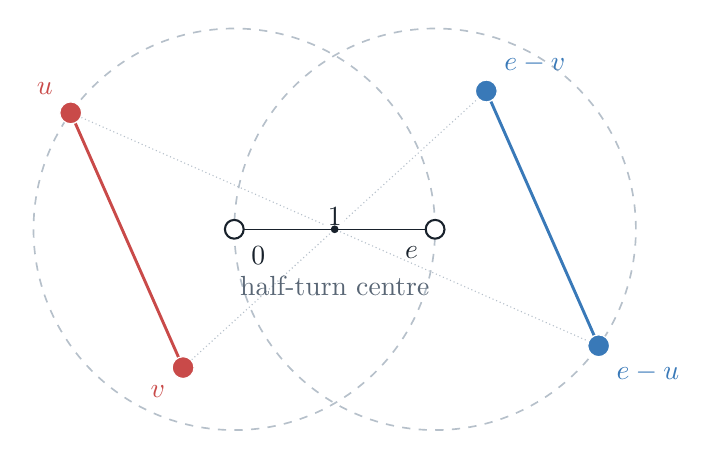
\begin{tikzpicture}[scale=2.55,
  root/.style={circle,draw=ink,fill=white,line width=.75pt,inner sep=2.4pt},
  red/.style={circle,fill=redpt,draw=white,line width=.45pt,inner sep=2.8pt},
  blue/.style={circle,fill=bluept,draw=white,line width=.45pt,inner sep=2.8pt}]
  \coordinate (O) at (0,0);
  \coordinate (E) at (1,0);
  \coordinate (u) at (-.8146,.5800);
  \coordinate (v) at (-.2550,-.6887);
  \coordinate (up) at (1.8146,-.5800);
  \coordinate (vp) at (1.2550,.6887);
  \draw[linegray,dashed,line width=.6pt] (O) circle (1);
  \draw[linegray,dashed,line width=.6pt] (E) circle (1);
  \draw[redpt,line width=1.05pt] (u)--(v);
  \draw[bluept,line width=1.05pt] (up)--(vp);
  \draw[linegray,densely dotted] (u)--(up) (v)--(vp);
  \draw[ink,line width=.55pt] (O)--node[above,fill=white,inner sep=1pt] {$1$}(E);
  \node[root,label={[ink]below right:$0$}] at (O) {};
  \node[root,label={[ink]below left:$e$}] at (E) {};
  \node[red,label={[redpt]above left:$u$}] at (u) {};
  \node[red,label={[redpt]below left:$v$}] at (v) {};
  \node[blue,label={[bluept]below right:$e-u$}] at (up) {};
  \node[blue,label={[bluept]above right:$e-v$}] at (vp) {};
  \fill[ink] (.5,0) circle (.55pt);
  \node[muted] at (.5,-.28) {half-turn centre};
\end{tikzpicture}
\caption{The unique normalized extremizer $X_*$.  The dashed circles are
the two unit child disks; each sibling segment has length $\cstar$.}
\label{fig:extremizer}
\end{figure}

This is a physical configuration.  Both $x$-coordinates of $u,v$ are
negative, whereas the blue children have $x$-coordinate greater than $1$.
Every non-root red--blue horizontal separation therefore exceeds $1$, and
the root--child inequalities follow as well.

Four distances reveal why this point is special:
\[
 A=|e-u|,\qquad B=|e-2u|,\qquad C=|e-u-v|,\qquad D=|e-2v|.
\]
They obey three balance identities
\begin{align}
 B+D&=2\cstar(2\cstar-1),\label{eq:bal1}\\
 A+C&=3\cstar b+\cstar^2-1,\label{eq:bal2}\\
 2B&=(\cstar+1)b+3\cstar^2-2\cstar+1.\label{eq:bal3}
\end{align}
These are exactly the zero-score equations for the three mechanisms of
Section~\ref{sec:intuition}: four children against four children; a sibling
edge against a full rooted triangle; and a root--child edge against a full
rooted triangle.  Half-turn symmetry duplicates the latter two, so five
moves tie at zero.  Moving the children to defeat the four-child move
improves one of the edge--triangle moves, and conversely; the endpoint is
the nonsmooth balance point of all three pressures.

\section{The obstruction: no constant below \texorpdfstring{$\sstar$}{s*}}
\label{sec:obstruction}

At the configuration $X_*$ of Figure~\ref{fig:extremizer}, precisely the
supports
\[
 57,\quad 75,\quad 66,\quad 67,\quad 76
\]
have score zero; every other support has negative score.

\begin{theorem}[exact obstruction]\label{thm:obstruction}
$F_{\sstar}(X_*)=0$, and $F_s(X_*)<0$ for every $s<\sstar$.  Consequently
$\theta_6\ge\sstar$.
\end{theorem}

\begin{proof}
The radii of the five displayed moves are explicit, and the three
identities \eqref{eq:bal1}--\eqref{eq:bal3} make their scores zero.

For each of the $49$ supports the remaining choice of radii is a linear
program.  One exhibits a feasible dual for one representative of every
colour-swap pair.  The active duals have value zero.  Exact rational
interval substitution in \eqref{eq:isolation-box} makes every inactive dual
value smaller than $-0.0264$.  Hence no hidden support has positive score
and $F_{\sstar}(X_*)=0$.

If $s<\sstar$, the same configuration remains admissible, since its sibling
length is $2\sstar>2s$.  Every move contains both colours, hence has
diameter at least $1$, so its score at $s$ is strictly smaller than its
score at $\sstar$.  Taking the maximum over the $49$ supports gives
$F_s(X_*)<0$.
\end{proof}

This is an exact obstruction, not a numerical candidate.  What remains is
to prove that no other configuration is worse.

\section{Nine moves suffice}\label{sec:nine}

The converse does not need all $49$ supports.  We use only
\begin{equation}\label{eq:nine-supports}
 \boxed{66,\ 67,\ 76,\ 17,\ 71,\ 37,\ 57,\ 73,\ 75.}
\end{equation}
Their roles are easier to remember than their masks.

\begin{center}
\begin{tabularx}{0.92\textwidth}{@{}lY@{}}
\toprule
support(s)&geometric role\\
\midrule
$66$&the four children\\
$67,76$&a sibling pair against the full opposite rooted triangle\\
$17,71$&one root against the full opposite rooted triangle\\
$37,57,73,75$&a root--child edge against the full opposite triangle\\
\bottomrule
\end{tabularx}
\end{center}

For an arbitrary configuration write the red children as $p_1,p_2$ and pull
the blue children back to the same unit disk by writing their actual
locations as $e-w_1,e-w_2$.  Thus
\[
 |p_i|\le1,\quad|w_j|\le1,\quad
 L:=|p_1-p_2|\ge\cstar,\quad M:=|w_1-w_2|\ge\cstar,
\]
and we set
\[
 r_i=|p_i|,\quad b_i=|w_i|,\quad B_{ij}=|e-p_i-w_j|,\quad
 a_i=\frac{r_i+b_i}{2}.
\]
Here $B_{ij}$ is the actual distance from red child $p_i$ to blue child
$e-w_j$.

\begin{theorem}[nine-packing theorem]\label{thm:nine}
At $s=\sstar$, every admissible configuration has a move of nonnegative
score among the nine supports \eqref{eq:nine-supports}.  Equality is
possible only at $X_*$, up to reflection in the root line, interchange of
the colours, and relabelling of the two children within either colour.
\end{theorem}

The proof is a failure tree whose purpose is to turn the many possible
active diameter constraints into three scalar inequalities.

\begin{figure}[ht]
\centering
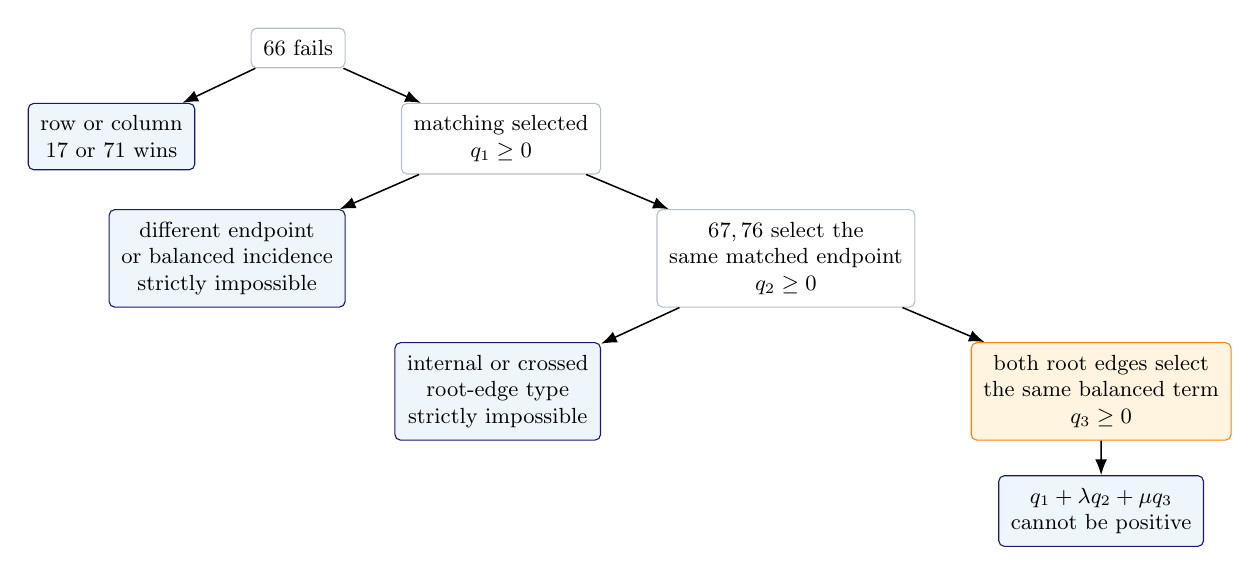
\begin{tikzpicture}[scale=.88,transform shape,
 node distance=5mm and 8mm,
 every node/.style={font=\small,align=center},
 box/.style={draw=linegray,rounded corners=2pt,fill=white,inner sep=5pt},
 good/.style={draw=MidnightBlue,rounded corners=2pt,fill=cool,inner sep=5pt},
 bad/.style={draw=BurntOrange,rounded corners=2pt,fill=warm,inner sep=5pt},
 arr/.style={-{Latex[length=2mm]},line width=.55pt}]
 \node[box] (a) {$66$ fails};
 \node[good,below left=of a] (ar) {row or column\\$17$ or $71$ wins};
 \node[box,below right=of a] (am) {matching selected\\$q_1\ge0$};
 \node[good,below left=of am] (si) {different endpoint\\or balanced incidence\\strictly impossible};
 \node[box,below right=of am] (se) {$67,76$ select the\\same matched endpoint\\$q_2\ge0$};
 \node[good,below left=of se] (ri) {internal or crossed\\root-edge type\\strictly impossible};
 \node[bad,below right=of se] (re) {both root edges select\\the same balanced term\\$q_3\ge0$};
 \node[good,below=of re] (co) {$q_1+\lambda q_2+\mu q_3$\\cannot be positive};
 \draw[arr] (a)--(ar);
 \draw[arr] (a)--(am);
 \draw[arr] (am)--(si);
 \draw[arr] (am)--(se);
 \draw[arr] (se)--(ri);
 \draw[arr] (se)--(re);
 \draw[arr] (re)--(co);
\end{tikzpicture}
\caption{The failure tree.  Blue boxes are strict exits.  The only
surviving path produces the three active slacks of $X_*$.}
\label{fig:failure-tree}
\end{figure}

\subsection{First branch: the four-child minimax}

Give each sibling pair radii adding to its actual side length, and write
the two radius splits as $x\in[L-1,1]$, $y\in[M-1,1]$.  Minimizing the four
affine red--blue diameter terms over this rectangle gives an elementary
alternative: if support $66$ has negative score, then at least one of the
following holds.
\begin{align}
 B_{i1}+B_{i2}&\ge2+2(\cstar-1)L+(2\cstar-1)M,&&\text{some row }i,\label{eq:row}\\
 B_{1j}+B_{2j}&\ge2+(2\cstar-1)L+2(\cstar-1)M,&&\text{some column }j,\label{eq:column}\\
 B_{11}+B_{22}&\ge(2\cstar-1)(L+M),\label{eq:matching-a}\\
 B_{12}+B_{21}&\ge(2\cstar-1)(L+M).\label{eq:matching-b}
\end{align}
The exact minimax identity is proved in Appendix~\ref{app:routing}.  Its
other vertices cannot cause failure: a single entry would have to exceed
$3$, and a same-colour term is short by at least $\cstar^2+2\cstar-4>0$.

A row or column alternative is rescued by support $17$ or $71$; this is
Lemma~\ref{lem:row-rescue}, proved by a rational tangent bound with margin
greater than $0.32$.  We may therefore relabel the children so that
\eqref{eq:matching-a} holds, and retain its exact slack
\begin{equation}\label{eq:qM}
 q_M:=B_{11}+B_{22}-(2\cstar-1)(L+M)\ge0 .
\end{equation}
Since $L+M\ge2\cstar$, we obtain the slightly weaker but more convenient
\begin{equation}\label{eq:q1}
 q_1:=B_{11}+B_{22}-2\cstar(2\cstar-1)\ge q_M\ge0 .
\end{equation}

\subsection{Second branch: the two sibling--triangle moves}

For a rooted triangle with child radii $r_1,r_2$ and side $L$, use its
canonical tangent radii
\begin{equation}\label{eq:canonical}
 \alpha_0=\frac{r_1+r_2-L}{2},\qquad
 \alpha_1=\frac{r_1+L-r_2}{2},\qquad
 \alpha_2=\frac{r_2+L-r_1}{2},
\end{equation}
which are nonnegative and at most $1$; write $\beta_j$ for the analogous
blue radii.

The one-dimensional radius minimax for support $67$ says that a failure
witness is either an \emph{endpoint} term or a \emph{balanced} pair of
diameter terms; root-labelled and same-colour terms are automatically too
short.  The same holds for $76$.

Fixing the matching in \eqref{eq:matching-a} leaves a finite incidence
problem.  Endpoint/endpoint incidences have six orbits: two coincident, two
adjacent, two disjoint.  The coincident orbit lying on the selected
matching is the desired one.  Both disjoint orbits are excluded by a single
matching-independent triangle estimate; the two adjacent orbits have
separate exact tangent certificates; and the off-matching coincident orbit
is strictly excluded by a lens certificate
(Section~\ref{sec:certificates}).

If at least one witness is balanced there are eight endpoint/balanced and
seven balanced/balanced orbits.  Eleven are excluded by the two-point
rational tangent lemma of Appendix~\ref{app:tangent}; the remaining four
are strict lens inequalities.  Hence both sibling--triangle failures select
the same endpoint on the chosen matching; call it $B_{11}$.

Adding the two exact endpoint-failure inequalities and using $L+M\ge2\cstar$
gives
\begin{equation}\label{eq:q2}
 q_2:=B_{11}-\frac{(\cstar-1)a_1+(\cstar+1)a_2+3\cstar^2-3\cstar+2}{2}\ge0 .
\end{equation}
The finite incidence check is essential: a balanced witness cannot simply
be renamed an endpoint witness.

\subsection{Third branch: the two root-edge moves}

Keep the two individual endpoint inequalities that produced \eqref{eq:q2},
and consider the root--child edge opposite the selected child together with
the full opposite triangle.  Its radius minimax initially has sixteen
labelled terms; triangle inequalities reduce them pointwise to three types:
an internal term, a balanced $(1,1)$ term, and a balanced $(1,2)$ term.

The internal term has a rational tangent separator with margin greater than
$5$.  The $(1,2)$ term has a four-variable outward-rounded certificate.
Consequently both colour directions must use the $(1,1)$ balanced term, and
adding those two failure inequalities yields
\begin{equation}\label{eq:q3}
 q_3:=A_1+C_1-\bigl((\cstar-1)a_1+3\cstar a_2+\cstar^2-\cstar\bigr)\ge0,
\end{equation}
where
\[
 A_1=\frac{|e-p_1|+|e-w_1|}{2},\qquad
 C_1=\frac{B_{12}+B_{21}}{2}.
\]

Failure of all nine moves therefore forces \eqref{eq:q1}, \eqref{eq:q2} and
\eqref{eq:q3}.  At $X_*$ all three are equalities: they are precisely
\eqref{eq:bal1}--\eqref{eq:bal3}.

\section{Why the three failures are incompatible}\label{sec:weighted}

There are exact positive algebraic numbers
\begin{align*}
 \lambda&=0.0894764254088637022746561625951140\ldots,\\
 \mu&=0.9288383388753901930144096356553482\ldots,
\end{align*}
defined by the two tangential stationarity equations at $(u,v)$; their
short exact definition is Appendix~\ref{app:weights}.  Put
\begin{equation}\label{eq:W-def}
 \W(P,W)=q_1+\lambda q_2+\mu q_3 .
\end{equation}
Positivity of the coefficients matters: the failure tree gives
$\W(P,W)\ge0$.

\begin{lemma}[weighted geometric lemma]\label{lem:weighted}
For all ordered sibling pairs $P=(p_1,p_2)$ and $W=(w_1,w_2)$ in the unit
disk with sibling lengths at least $\cstar$,
\begin{equation}\label{eq:W-nonpositive}
 \W(P,W)\le0 .
\end{equation}
Equality holds only when $P=W=(u,v)$, or when both pairs are their common
reflection in the root line.
\end{lemma}

The lemma has two parts.  The first is a one-pair inequality,
\begin{equation}\label{eq:self}
 \W(X,X)\le0,
\end{equation}
with equality only at $(u,v)$ or its reflection.  The second is the mixed
contraction: when both sibling lengths equal $\cstar$,
\begin{equation}\label{eq:contraction}
 9\W(P,W)\le4\bigl\{\W(P,P)+\W(W,W)\bigr\}.
\end{equation}
Together \eqref{eq:self} and \eqref{eq:contraction} give
\eqref{eq:W-nonpositive} on the chord boundary.

\subsection{Reduction to the chord boundary}

Expanding \eqref{eq:W-def},
\begin{equation}\label{eq:W-expanded}
 \W(P,W)=(1+\lambda)B_{11}+B_{22}+\mu(A_1+C_1)-Ua_1-Va_2-K,
\end{equation}
with
\begin{align*}
 U&=(\cstar-1)\left(\frac\lambda2+\mu\right),\\
 V&=\frac{\cstar+1}{2}\lambda+3\cstar\mu,\\
 K&=2\cstar(2\cstar-1)+\frac\lambda2(3\cstar^2-3\cstar+2)+\mu(\cstar^2-\cstar).
\end{align*}
Move $p_2$ inward along its ray until $|p_1-p_2|=\cstar$.  The positive
distance terms in \eqref{eq:W-expanded} change at total speed at most
$1+\mu/2$, whereas the radial penalty changes at speed $V/2$, and exact
arithmetic gives
\[
 \frac V2-1-\frac\mu2>\frac12 .
\]
So the inward move strictly increases $\W$; the same applies to $w_2$.
Proving the bound after the two moves proves it before them, and equality
forces both original sibling lengths to equal $\cstar$.

\subsection{What the contraction controls}

Put $x_i=e-2p_i$ and $y_i=e-2w_i$, and define the midpoint loss and the
crossed mismatch
\[
 \delta(x,y)=\frac{|x|+|y|-|x+y|}{2}\ge0,\qquad
 \chi=\frac{|x_1+y_2|+|y_1+x_2|-|x_1+x_2|-|y_1+y_2|}{4}.
\]
A direct cancellation turns \eqref{eq:contraction} into
\begin{equation}\label{eq:mechanism-H}
 \frac{9\W(P,W)-4\W(P,P)-4\W(W,W)}{8}
 =\frac{\W(P,W)}{8}-(1+\lambda)\delta(x_1,y_1)-\delta(x_2,y_2)+\mu\chi\le0 .
\end{equation}
The two $\delta$ terms reward alignment of the two colours.  The only term
that can oppose them is the crossed mismatch $\chi$, and the small residual
$\W/8$ supplies exactly the extra control needed at the extremizer.  This
is the global mechanism behind the half-turn symmetry.

\subsection{The equality case}

The global contraction certificate is strict outside a small box in the one
chart containing $(P,W)=((u,v),(u,v))$.  In that box the two height
variables are strictly increasing, so a maximum lies on the two
unit-circle faces.  The remaining four-variable Hessian is negative
definite, so the contraction expression is strictly concave there.  It is
symmetric under $P\leftrightarrow W$, hence its unique maximizer lies on
the diagonal $P=W$.  On that diagonal the left-hand side of
\eqref{eq:mechanism-H} equals $\W(P,P)/8$, and the equality statement
follows from the self inequality \eqref{eq:self}.

\begin{proof}[Proof of Theorem~\ref{thm:nine}]
Suppose first that all nine selected scores are negative.  The failure tree
gives $q_1,q_2,q_3\ge0$ and therefore $\W(P,W)\ge0$, while
Lemma~\ref{lem:weighted} gives $\W(P,W)\le0$.  Equality is forced
throughout, so $P=W=(u,v)$ up to reflection and relabelling.  At that
configuration five selected moves have score zero, contradicting the
assumed strict failure.

For the equality statement, assume instead that every selected score is
nonpositive.  The row, nonactive-incidence, internal and $(1,2)$
separators are all strict, so the same failure tree still reaches
$q_1,q_2,q_3\ge0$, and equality in Lemma~\ref{lem:weighted} again forces
the displayed half-turn configuration.
\end{proof}

\section{Deduction of the optimal constant}\label{sec:optimality}

\begin{theorem}\label{thm:main-body}
The optimal two-colour six-point constant is
\[
 \boxed{\theta_6=\sstar=0.693306421825904872690678414403710951\ldots}
\]
and the normalized equality configuration is the half-turn configuration of
Figure~\ref{fig:extremizer}, up to its evident symmetries.
\end{theorem}

\begin{proof}
Theorem~\ref{thm:obstruction} gives $\theta_6\ge\sstar$; it remains to show
strict positivity above $\sstar$.

At the endpoint, Theorem~\ref{thm:nine} gives $m_6(\sstar)\ge0$, while the
obstruction gives the reverse inequality.  Hence $m_6(\sstar)=0$, and the
equality statement identifies exactly where this occurs.

Fix $s>\sstar$.  Its admissible configuration space is compact and is a
closed subset of the space admissible at $\sstar$.  The best score among
the nine moves is continuous in the six centres, being the maximum of
finitely many compact linear-program optima.  By Theorem~\ref{thm:nine} it
is nonnegative at $\sstar$, and its only zeros have sibling length
$2\sstar$; such configurations are not admissible at $s$, where the sibling
length must be at least $2s>2\sstar$.  Compactness therefore gives a
uniform positive minimum on the $s$-admissible space.

Finally the score of every fixed move increases with $s$, because the
coefficient of its positive diameter in \eqref{eq:score} decreases.  Hence
the best nine-move score at parameter $s$ is at least its already positive
value computed at $\sstar$, so $m_6(s)>0$ for every $s>\sstar$ and
$\theta_6\le\sstar$.
\end{proof}

\section{The finite certificates}\label{sec:certificates}

This section states exactly where a computer is used.  No optimizer, random
sample, or floating-point sign is part of the proof.  Each
computer-assisted claim is a universal inequality on an explicitly covered
compact domain.

\subsection{The common chord charts}

After the radial reductions a sibling pair has exact length $\cstar$.  In a
local frame it can be written
\begin{equation}\label{eq:lens-basic}
 x_1=a\,n+h\,n^\perp,\qquad x_2=(a-\cstar)\,n+h\,n^\perp,
\end{equation}
and the unit-disk condition is exactly
\[
 \cstar-1\le a\le1,\qquad |h|\le\sqrt{1-\max\{a^2,(a-\cstar)^2\}}.
\]
Two charts remove the maximum and all trigonometric functions.  Put
$d=1-\cstar/2$ and take $t,q\in[0,1]$.  On the two halves of the lens use
\[
 a=1-dt^2 \quad\text{or}\quad a=\cstar-1+dt^2,\qquad
 H=t\sqrt{2d-d^2t^2},\qquad h=(2q-1)H .
\]
For the direction use the rational unit-circle chart
\begin{equation}\label{eq:circle-chart}
 n=\left(\varepsilon\frac{1-z^2}{1+z^2},\ \frac{2z}{1+z^2}\right),
 \qquad\varepsilon\in\{-1,1\}.
\end{equation}
Global reflection lets the first pair use $z\in[0,1]$; the second uses
$z\in[-1,1]$.  The two lens halves and the two signs for each pair give
$16$ six-dimensional boxes, and
\eqref{eq:lens-basic}--\eqref{eq:circle-chart} cover the entire chord
domain, including overlapping boundaries.

\subsection{Outward arithmetic and the covering argument}

At precision $N$ an interval is stored as $[m/2^N,\,n/2^N]$ with
$m,n\in\Z$.  Addition is exact; products and quotients use integer floor
and ceiling; square-root endpoints use integer square root.  Every
operation is therefore rounded outward.  The algebraic constants
$\cstar,\lambda,\mu$ enter only through rational intervals already proved
to contain them.

On each box the verifier evaluates a pointwise upper function --- either the
natural interval extension or a norm-tangent majorant --- together with an
automatic-differentiation mean-value bound.  On smaller unresolved boxes it
may also use the rigorous Taylor estimate
\begin{equation}\label{eq:taylor-bound}
 f(x)\le f(m)+\sum_i|f_i(m)|h_i+\frac12\sum_{i,j}\sup_B|f_{ij}|\,h_ih_j,
\end{equation}
where $m$ is the box midpoint and $h_i$ its half-width.  If an upper bound
is negative, that box is finished.  If a derivative has a fixed sign, the
maximum moves to the corresponding face.  Otherwise the box is bisected.
Every step replaces a box by an exact cover of itself, so a finite list of
negative leaves proves the inequality on the whole domain; the split choice
affects running time but not validity.  If an optional second-derivative
expression overflows the integer range, or a rounded derivative denominator
meets zero, that Taylor estimate is discarded and the already valid
first-order bound is subdivided --- such a box is never accepted as a leaf.

For the contraction, positive norms also use
\[
 |v|\le\frac{|v|^2+\rho^2}{2\rho},
\]
and negative norms use a supporting linear functional.  The dyadic $\rho$
and the supporting direction are chosen at the centre of the current box;
both inequalities are valid at every point of the box.

\subsection{Strict routing inequalities}

The routing proof uses the following exact separators.  In every row the
displayed linear combination has nonnegative coefficients on the failure
slacks; except for a zero $q_M$ coefficient in four tangent rows all are
positive, and in those four rows the other two coefficients are positive.
A strict negative upper bound therefore always rules out simultaneous
failure.

\begin{center}
\begin{tabularx}{\textwidth}{@{}YYl@{}}
\toprule
branch&proof method&certified margin\\
\midrule
four-child row/column&rational two-point tangents&$>0.321$\\
endpoint, disjoint&triangle inequality&$>0.14$\\
endpoint, adjacent $(0,1)$&rational two-point tangents&$>0.00157$\\
endpoint, adjacent $(0,2)$&rational two-point tangents&$>0.00585$\\
$11$ sibling-incidence cells&rational two-point tangents&$>0.17$\\
$4$ sibling-incidence cells&exact six-variable lens cover&$>4.14\cdot10^{-8}$\\
off-matching coincident endpoint&exact six-variable lens cover&$>1.18\cdot10^{-5}$\\
root-edge internal&rational two-point tangents&$>5$\\
root-edge $(1,2)$&exact four-variable lens cover&$>6.47\cdot10^{-5}$\\
\bottomrule
\end{tabularx}
\end{center}

The structurally delicate strict sibling case is the endpoint/balanced
orbit $(E0,S0)$.  Its positive separator is
\begin{align}\label{eq:hard-sibling}
 F={}&17B_{11}+5B_{22}+3B_{12}
 -3\bigl\{(\cstar-1)r_1+(\cstar+1)r_2\bigr\}\notag\\
 &-\frac92\bigl\{(\cstar-1)b_1+(\cstar+1)b_2\bigr\}
 -9+\frac{59}{2}\cstar-\frac{85}{2}\cstar^2 .
\end{align}
The radial estimates first put both sibling pairs on their chord floors;
there, where $L=M=\cstar$, the positive combination $5q_M+9q_E+6q_S$
simplifies to the displayed $F$, where $q_E$ is the exact red endpoint
slack and $q_S$ the colour-reversed balanced slack whose two endpoints both
target red child~$1$.  The exact lens cover proves $F<0$.  The other four
compiled cases are handled in the same way.

The frozen $40$-bit replay covers $16$ charts for each of the five compiled
cases, hence $80$ charts.  It processes $13{,}269{,}127$ boxes;
$6{,}492{,}866$ leaves are certified negative, and every other processed
box is either moved to a monotone face or split into an exact cover.  The
run makes $751{,}477$ optional Hessian attempts, of which $260$
under-resolved attempts are discarded and fall back to subdivision,
certifying no leaf.  The closest negative upper endpoint over all five
cases is $-4.1431121644563973\cdot10^{-8}$.

The root-edge $(1,2)$ separator first uses scalar norm tangents to remove
both rotation angles analytically, leaving four shape variables.  Its
$180$-bit replay has $182{,}403$ processed boxes and largest negative upper
endpoint $-6.479780941431465\cdot10^{-5}$.

\subsection{The self inequality}

For $X=(p_1,p_2)$, expansion gives
\begin{align*}
 \W(X,X)={}&(1+\lambda)|e-2p_1|+|e-2p_2|\\
 &+\mu\bigl\{|e-p_1|+|e-p_1-p_2|\bigr\}-U|p_1|-V|p_2|-K .
\end{align*}
Because $V-(2+\mu)>1.0417$, moving $p_2$ inward strictly raises this
quantity until $|p_1-p_2|=\cstar$.  On that boundary write
$r=|p_1|$, $b=|p_2|$, $t=(p_1)_x/r$.  The feasible radii are parameterized
by a square,
\[
 r=\cstar-1+(2-\cstar)u,\qquad b=(\cstar-r)(1-v)+v,\qquad 0\le u,v\le1,
\]
and the chord equation gives the two possible horizontal coordinates of
$p_2$, the smaller of which always gives the larger value of $\W$.  This
turns the assertion into one explicit function on $[0,1]^2\times[-1,1]$.

The $180$-bit global cover has $169{,}285$ strict leaves and one local box,
with largest certified negative upper endpoint
$-2.2320712193774615\cdot10^{-8}$.  On the local box, exact
differentiation first puts $|p_1|=1$; a cover by $201$ rectangles then
proves
\[
 \W_{vv}<-0.0870,\qquad \W_{tt}<-3.5406,\qquad \det D^2\W>0.00400 .
\]
Hence the remaining two-variable function is strictly concave.  The
algebraic point $(u,v)$ has value and gradient zero, so it is the unique
maximum.  This proves \eqref{eq:self} and its equality statement.

\subsection{The mixed contraction}

The identity \eqref{eq:mechanism-H} is evaluated on the same $16$ lens
charts.  After expansion it has six norms with positive coefficients and
ten with negative coefficients; on each box the verifier replaces a
positive norm by $|z|\le(|z|^2+\rho^2)/(2\rho)$ and a negative norm by a
supporting linear functional, both valid pointwise on the box.  The
resulting smooth majorant is then bounded by the mean-value and Taylor
rules above.

Fifteen charts are strictly negative.  The equality chart leaves one
rational local box, where exact first derivatives put both height
parameters on their top faces, an exact subdivision proves the
four-variable Hessian negative definite, and the symmetry-and-diagonal
argument following \eqref{eq:mechanism-H} finishes using the self lemma.

For a reproducible replay the equality chart is cut at four exact dyadic
midplanes into $16$ closed prefix boxes; a separate integer check proves
their union is the entire chart, and the boxes overlap only on shared
midpoint faces.  The $15$ ordinary charts and these $16$ prefixes report

\begin{center}
\begin{tabular}{@{}lr@{}}
\toprule
processed boxes&$303{,}467{,}033$\\
strict negative leaves&$151{,}733{,}531$\\
local equality leaves&$1$\\
second-order bound attempts&$15{,}536{,}510$\\
\bottomrule
\end{tabular}
\end{center}

\noindent
The closest accepted strict upper endpoint is exactly one negative
fixed-point unit,
\[
 -2^{-40}=-9.0949470177292824\cdot10^{-13}<0 .
\]
On the remaining local leaf the derivative lower margin is $0.0124096$, and
the negative-definiteness proof has $32{,}768$ interval-LDL leaves with
least pivot margin $0.0328339$.

Every reported decimal margin is a readable rendering of an exact rational
or dyadic endpoint.  All sign decisions use the corresponding integer
comparisons.

\section{From the six-point constant to the density threshold}
\label{sec:transfer}

We record the two steps that turn Theorem~\ref{thm:main-body} into
Theorem~\ref{thm:B}.  Both are formalized in full
(Section~\ref{sec:lean}).

\begin{definition}[straight measure]
A Borel measure $\mu$ on $\R^2$ is \emph{straight} if
$\mu(A)\le\diam A$ for every measurable $A$.
\end{definition}

\begin{definition}[Besicovitch pair condition]\label{def:bpc}
$\mathrm{BPC}(\beta)$ holds if for every straight measure $\mu$ there is
$\tau>0$ such that for every scale $\sigma>0$ there is $\delta>0$ with the
following property.  Whenever $E_1,E_2$ are nonempty measurable sets with
$0<\dist(E_1,E_2)<\delta$ and
\[
 \mu(B(x,r))>2\beta r\qquad\text{for all }x\in E_1\cup E_2,\ 0<r<\sigma,
\]
there is an open set $V$ meeting both $E_1$ and $E_2$ with
\[
 \mu\bigl(V\setminus(E_1\cup E_2)\bigr)>\tau\diam V .
\]
\end{definition}

\begin{proposition}[six-point transfer]\label{prop:transfer}
Let $0<s<1$ and suppose every configuration admissible at $s$ admits a move
of nonnegative score, i.e.\ $m_6(s)\ge0$.  Then $\mathrm{BPC}(\beta)$ holds
for every $\beta>s$.
\end{proposition}

The proof extracts two children near each of two approximate closest points
of $E_1$ and $E_2$, normalizes the roots to distance $1$, applies the
six-point property, and absorbs the normalization error using the strict
inequality $\beta>s$.  Straightness turns the mass in each root ball into a
sibling pair of large separation; the physical packing then contradicts
straightness by inclusion--exclusion unless the required leaking open set
$V$ exists.  Only six centres are used.

\begin{proposition}[pair condition to rectifiability]\label{prop:rect}
If $\mathrm{BPC}(\beta)$ holds with $0<\beta<1$, then every Borel set of
finite $\HH^1$ measure whose lower density is at least $\gamma>\beta$
almost everywhere is countably $1$-rectifiable.
\end{proposition}

This is the classical route: decompose into rectifiable and purely
unrectifiable parts, localize at a density point of the purely
unrectifiable part to obtain a straight measure, apply
Definition~\ref{def:bpc} to a maximal disjoint selection, and use continuum
surgery together with the fact that a continuum of finite $\HH^1$ measure
is rectifiable to produce a rectifiable subset of positive measure ---
contradicting pure unrectifiability.

\begin{proof}[Proof of Theorem~\ref{thm:B}]
Let $c>\sstar$ and choose $\beta$ with $\sstar<\beta<c$.  By
Theorem~\ref{thm:main-body}, $m_6(\sstar)\ge0$, so
Proposition~\ref{prop:transfer} gives $\mathrm{BPC}(\beta)$, and
Proposition~\ref{prop:rect} shows that $c$ forces rectifiability.  Since
$c>\sstar$ was arbitrary, $\sigma_1(\R^2)\le\sstar$.
\end{proof}

\begin{remark}
The transfer needs only $\beta>\sstar$, never the endpoint assertion
$\mathrm{BPC}(\sstar)$ itself; the infimum in the definition of $\sigma_1$
supplies the non-strict conclusion.  This is why the endpoint case of the
six-point problem --- the hardest part of the paper --- has to be settled
exactly, while the pair condition may be used with room to spare.
\end{remark}

\section{Formalization in Lean 4}\label{sec:lean}

The argument is being formalized in Lean~4 with Mathlib, pinned to
\texttt{v4.32.0}, in the repository accompanying this paper.  The target
statements are
\begin{center}
\texttt{Besicovitch.sigma\_one\_plane\_le\_s\_star} \quad and \quad
\texttt{Besicovitch.sStar\_le\_6934\_div\_10000},
\end{center}
namely $\sigma_1(\R^2)\le\sstar$ and $\sstar\le0.6934$.  All definitions
occurring in these statements --- lower density, countable
$1$-rectifiability, the threshold $\sigma_1$, and the endpoint $\sstar$ as
the exact isolated radical system of Section~\ref{sec:number} --- are
transparent and are compared recursively against an independent copy, so
neither the statement of the theorem nor the meaning of the constant can
drift during the proof.  The verification gates exclude
\texttt{native\_decide}, \texttt{Lean.ofReduceBool}, and custom axioms; the
only axioms permitted in the finished theorem are \texttt{propext},
\texttt{Quot.sound}, and \texttt{Classical.choice}.  Hashes, program exit
codes, and floating-point samples are not proof objects: Bernstein
conversion and outward-rounded interval arithmetic are themselves
implemented and proved sound inside Lean.

At the time of writing, the entire transfer chain of
Section~\ref{sec:transfer} is complete and free of \texttt{sorry},
including the geometric-measure-theory results absent from Mathlib
(straight decomposition, continuum surgery, finite-length continuum
rectifiability, density localization, uniform density on compacta), which
are proved locally rather than assumed.  The numerical bound
$\sstar\le0.6934$ is likewise discharged.  The remaining work is confined
to the endpoint inequality of Section~\ref{sec:weighted} --- in the
formalization, the coordinate-free statement
\texttt{WeightedGeometricBound} and its chart form
\texttt{WeightedLensChartBound}.  Until that hole is closed the Lean
development must not be read as a completed proof; its current state is
tracked in the repository's development plan.

\section{Concluding remarks}

Two features of this result deserve emphasis.

First, the constant is \emph{optimal for its instance}.  Theorem~\ref{thm:A}
is not an estimate that further effort on the same six-point problem could
improve: $\theta_6$ is exactly $\sstar$, and the extremal configuration is
unique.  Any further progress toward $1/2$ along this route must come from
a genuinely larger finite problem --- more centres, or a different grouping
--- and not from sharpening the present analysis.

Second, the extremizer is informative.  It is a half-turn pair of chords of
length $\cstar$ pressed against the boundaries of their unit disks, at
which three structurally different packing mechanisms tie simultaneously.
Any candidate finite problem that hopes to reach below $\sstar$ must
possess moves that break at least one of those three ties, and the balance
identities \eqref{eq:bal1}--\eqref{eq:bal3} say precisely which ones.

\appendix

\section{The routing algebra}\label{app:routing}

\subsection{The exact two-by-two minimax}

Let two same-colour pairs have centre distances $L,M\in[\cstar,2]$.  At a
score maximizer their two radius sums may be taken to be $L$ and $M$:
raising an unsaturated radius by $\varepsilon$ raises the diameter by at
most $\varepsilon$, hence raises the score because $1-1/\cstar>0$; and the
same-colour two-ball primitive dominates either self-ball primitive
because $L,M>1$, so no hidden $2r_i$ term invalidates the increase.

Put $Q=L+M$ and write the red radii as $x,L-x$ and the blue radii as
$y,M-y$.  The cap $r_i\le1$ gives $L-1\le x\le1$ and $M-1\le y\le1$.
Minimizing the maximum of the four cross-diameter terms over this rectangle
and adjoining the same-colour terms gives exactly
\begin{align}\label{eq:minimax-full}
 \Delta_{66}=\max\Bigl\{&2L,\ 2M,\ Q+B_{ij}-2,\notag\\
 &\frac{Q+L-2+B_{i1}+B_{i2}}{2},\ \frac{Q+M-2+B_{1j}+B_{2j}}{2},\notag\\
 &\frac{Q+B_{11}+B_{22}}{2},\ \frac{Q+B_{12}+B_{21}}{2}
 \ :\ i,j=1,2\Bigr\}.
\end{align}
A quick proof is linear-programming duality: after centring the two split
intervals, a dual distribution on the four entries of the $B$-matrix has
vertices of four kinds --- one entry, two entries in a row, two in a
column, or two in a perfect matching --- and these are exactly the terms in
\eqref{eq:minimax-full}.  Equating a failed score to
$\Delta_{66}\ge\cstar Q$ gives \eqref{eq:row}--\eqref{eq:matching-b}.

The two omitted kinds are automatic.  In the worse ordering,
$\cstar Q-2L\ge\cstar(\cstar+2)-4>0$.  A single-entry offender would
require $B_{ij}\ge2+(\cstar-1)Q\ge2+2\cstar(\cstar-1)>3$, whereas
$B_{ij}\le1+r_i+b_j\le3$.

\subsection{The row/column rescue}

\begin{lemma}\label{lem:row-rescue}
If \eqref{eq:row} holds, support $17$ has nonnegative score.  If
\eqref{eq:column} holds, support $71$ has nonnegative score.
\end{lemma}

\begin{proof}
We prove the row statement; colour interchange gives the other.  If support
$17$ also failed, its only possible obstructing primitive would select one
of the two blue children; relabel it as child one.  We would then have
\begin{align*}
 |e-p-w_1|+|e-p-w_2|&\ge2+2(\cstar-1)L+(2\cstar-1)M,\\
 |e-w_1|&\ge\cstar-1+\frac{(\cstar-1)(b_1+M)+(\cstar+1)b_2}{2}.
\end{align*}
The root--root and same-colour primitives are strictly below the target,
and the root--child assertion follows from the canonical triangle radii
\eqref{eq:canonical}.  Let $q_R,q_E$ denote left side minus right side in
the two displayed inequalities; simultaneous failure makes both slacks
nonnegative.

Move $w_2$ inward along its ray.  On the region $M\ge\cstar$,
\[
 \frac{dM}{dt}\ge d_0:=\frac{\sqrt{\cstar^2-1}}{\cstar},
 \qquad (2\cstar-1)d_0>1,
\]
so both failure slacks increase until $M=\cstar$.  The first inequality may
also be weakened to $L=\cstar$, and convexity puts $|p|=1$.

For these reduced inequalities the positive combination $10q_R+9q_E$ is
bounded by applying $N\le(N^2+\rho^2)/(2\rho)$ three times, followed twice
by $2|z|\le\sigma+|z|^2/\sigma$, with rational tangent parameters
\[
 \rho_1=\frac{361}{125},\quad \rho_2=\frac{64}{25},\quad
 \rho_3=\frac{1937}{1000},\quad \sigma=\frac{601}{100},\quad
 \eta=\frac{567}{100}.
\]
The resulting function is convex in $(b_1,b_2)$, so only
$(1,1)$, $(1,\cstar-1)$, $(\cstar-1,1)$ need be checked; exact rational
substitution gives upper bounds below $-0.3228344$, $-0.3213815$ and
$-9.9505$ respectively.  In particular $10q_R+9q_E<-8/25$, contradicting
simultaneous failure.
\end{proof}

\subsection{The sibling and root-edge primitives}

The exact endpoint failure slacks used in the second branch are
\begin{align*}
 q_{ER}(i,j)&=L-1+B_{ij}+\beta_j-\cstar(L+T_B),\\
 q_{EB}(i,j)&=M-1+B_{ij}+\alpha_i-\cstar(M+T_P),
\end{align*}
where
\[
 T_P=\frac{r_1+r_2+L}{2},\qquad T_B=\frac{b_1+b_2+M}{2}.
\]
A balanced red-sibling witness selecting blue children $j,k$ has slack
\[
 q_{SR}(j,k)=\frac{L+B_{1j}+\beta_j+B_{2k}+\beta_k}{2}-\cstar(L+T_B),
\]
and the colour-reversed slack is
\[
 q_{SB}(i,k)=\frac{M+B_{i1}+\alpha_i+B_{k2}+\alpha_k}{2}-\cstar(M+T_P).
\]
A balanced witness using two different target children already gives one of
the two matching inequalities.  An endpoint cannot target the triangle
root, since
\[
 \cstar(L+T_B)-\bigl\{L-1+|e-p_i|+\beta_0\bigr\}
 \ge(\cstar-1)L+\Bigl(\cstar+\tfrac12\Bigr)M-2
 \ge2\cstar^2-\tfrac12\cstar-2>1 .
\]
A balanced root or root--child target is also impossible: its elementary
upper bound is at most $6$, while the necessary lower bound is
$4\cstar^2-\cstar>6$.  These observations leave exactly the incidence
orbits treated in Section~\ref{sec:nine}.

\section{The rational two-point tangent lemma}\label{app:tangent}

Let $x_1,x_2$ lie in the unit disk, put $t_i=|x_i|$ and $N_i=|e-2x_i|$, and
assume $|x_1-x_2|\ge\cstar$.  For $A_i,\rho_i,\sigma>0$ and $d_i\ge0$ put
$g_i=A_i/\rho_i$.  Then
\begin{equation}\label{eq:tangent-phi}
 A_1N_1+A_2N_2-d_1t_1-d_2t_2\le\max_{(u,v)\in V}\Phi(u,v),
\end{equation}
where $V=\{(1,1),(1,\cstar-1),(\cstar-1,1)\}$ and, with $s_1=u$, $s_2=v$,
\begin{align*}
 \Phi(u,v)&=\sum_{i=1}^2\frac{A_i}{2\rho_i}\bigl(1+\rho_i^2+4s_i^2\bigr)
   +\sigma+\frac{Q}{\sigma}-d_1u-d_2v,\\
 Q&=(g_1+g_2)(g_1u^2+g_2v^2)-g_1g_2\cstar^2 .
\end{align*}
Indeed, tangent each $N_i$ and observe
\[
 |g_1x_1+g_2x_2|^2=(g_1+g_2)(g_1t_1^2+g_2t_2^2)-g_1g_2|x_1-x_2|^2\le Q,
\]
then use $2\sqrt Q\le\sigma+Q/\sigma$.  The resulting upper bound is convex
on the radial polygon $0\le t_i\le1$, $t_1+t_2\ge\cstar$, whose relevant
vertices are exactly $V$.

The other elementary ingredient is midpoint convexity,
\begin{equation}\label{eq:B-midpoint}
 B_{ij}=\left|\frac{(e-2p_i)+(e-2w_j)}{2}\right|
 \le\frac{|e-2p_i|+|e-2w_j|}{2},
\end{equation}
which splits every rational separator into one red and one blue application
of \eqref{eq:tangent-phi}.  All tangent parameters in the accompanying
checker are rational; after the three radial evaluations, every sign is a
rational polynomial sign over \eqref{eq:isolation-box}.

\section{The exact weights}\label{app:weights}

Write $u=(x,y)$, $v=(z,t)$ with $y>0>t$ and $b=|v|$, and retain the
distances $A,B,C,D$ of Section~\ref{sec:number}.  Put
\[
 \kappa=\frac{1+b^2-\cstar^2}{2},\qquad R=\sqrt{b^2-\kappa^2},\qquad
 \rho=\frac{b(1-\kappa)}{R},\qquad z_b=bx-\rho y,
\]
\[
 D_b=\frac{4b-2z_b}{D},\qquad C_b=\frac{2b-z_b}{C}.
\]
The weights $\lambda,\mu$ are the unique solution of
\begin{equation}\label{eq:weight-system}
 \begin{pmatrix}
  2y/B & y/A+(y+t)/C\\[0.2em]
  -(\cstar+1)/2 & C_b-3\cstar
 \end{pmatrix}
 \begin{pmatrix}\lambda\\ \mu\end{pmatrix}
 =\begin{pmatrix}-2y/B-2t/D\\ -D_b\end{pmatrix}.
\end{equation}
These are the two first-order stationarity equations for
$q_1+\lambda q_2+\mu q_3$ at $(u,v)$.  The determinant is
$-0.8363707480\ldots$, bounded away from zero by exact intervals, and the
same calculation proves
\[
 \lambda>0,\qquad \mu>0,\qquad V-(2+\mu)>1 .
\]
Thus \eqref{eq:weight-system}, together with the exact algebraic point,
defines the weights without recourse to their decimal expansions.

\begin{thebibliography}{9}

\bibitem{Bes28} A.~S. Besicovitch,
\emph{On the fundamental geometrical properties of linearly measurable
plane sets of points}, Math. Ann. \textbf{98} (1928), 422--464.

\bibitem{Bes38} A.~S. Besicovitch,
\emph{On the fundamental geometrical properties of linearly measurable
plane sets of points II}, Math. Ann. \textbf{115} (1938), 296--329.

\bibitem{PT92} D.~Preiss and J.~Ti\v{s}er,
\emph{On Besicovitch's $\tfrac12$-problem},
J. London Math. Soc. (2) \textbf{45} (1992), 279--287.

\bibitem{DGMV24} C.~De Lellis, F.~Glaudo, A.~Massaccesi and D.~Vittone,
\emph{Besicovitch's $1/2$ problem and linear programming},
arXiv:2404.17536 (2024).

\bibitem{Falconer} K.~J. Falconer,
\emph{The Geometry of Fractal Sets}, Cambridge University Press, 1985.

\bibitem{Mattila} P.~Mattila,
\emph{Geometry of Sets and Measures in Euclidean Spaces},
Cambridge University Press, 1995.

\bibitem{Mathlib} The mathlib Community,
\emph{The Lean mathematical library}, CPP 2020, 367--381.

\end{thebibliography}

\end{document}
